\documentclass[border=7pt]{standalone}
\usepackage{fontspec,unicode-math}
\setmainfont{Noto Serif}
\setmathfont{STIXTwoMath-Regular.otf}
\usepackage{tikz}
\usetikzlibrary{arrows.meta,calc,patterns,decorations.pathreplacing,decorations.markings}
\tikzset{
  structure/.style={black,line width=.78pt,line join=round,line cap=round},
  potential/.style={black,line width=1.1pt,line join=round,line cap=round},
  level/.style={black,line width=1.04pt,line cap=butt},
  thinlevel/.style={black,line width=.66pt,line cap=butt},
  ax/.style={black,line width=.60pt,-{Latex[length=2mm,width=1.2mm]}},
  transition/.style={black,line width=.72pt,-{Latex[length=2mm,width=1.16mm]},shorten >=2pt,shorten <=2pt},
  dim/.style={black,line width=.66pt,{Latex[length=1.8mm,width=1mm]}-{Latex[length=1.8mm,width=1mm]}},
  annot/.style={font=\fontsize{11}{13}\selectfont,inner sep=1.6pt},
  panel/.style={font=\fontsize{13}{16}\selectfont\itshape,inner sep=1pt}
}
\pagestyle{empty}
\begin{document}
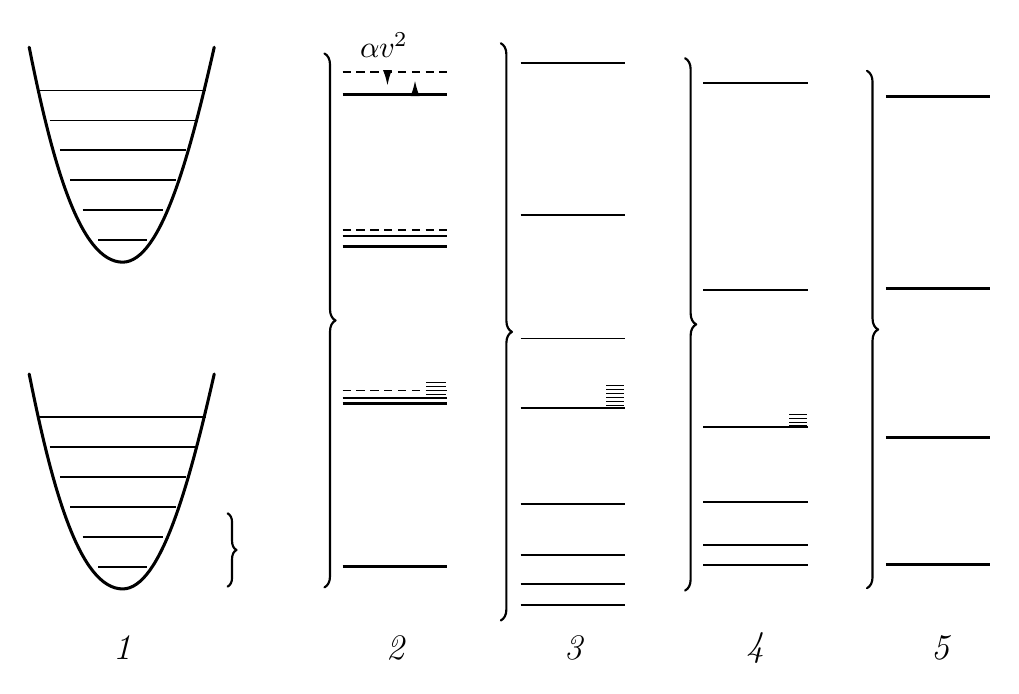
\begin{tikzpicture}[x=1cm,y=1cm]
% Original: two electronic terms -> vibrational -> J/K rotational -> hyperfine.
% This is a diagram of nested spectral scales, not measured level positions.
% Stage 1 two vertically stacked Morse-like wells, with six approximately equal spacings.
\foreach \v in {0,1} {
 \begin{scope}[shift={(0,{4.15*\v})}]
  \draw[potential] (.03,3.15) .. controls (.32,1.7) and (.67,.42) .. (1.22,.42)
    .. controls (1.70,.43) and (2.06,1.74) .. (2.38,3.15);
  \foreach \yy/\xa/\xb in {.70/.91/1.53,1.08/.71/1.73,1.46/.55/1.89,1.84/.42/2.02,2.22/.29/2.15,2.60/.16/2.28} {
    \draw[thinlevel] (\xa,\yy)--(\xb,\yy);
  }
 \end{scope}
}
% Author's rising brace between the two electronic-level wells, not connecting their minima.
\draw[structure,decorate,decoration={brace,mirror,amplitude=3.2pt}] (2.55,.45)--(2.55,1.38);
% Stage 2 split spectral scales; dashed harmonic anchors versus solid anharmonic levels.
\foreach \yy in {.70,2.77,4.77,6.70} {\draw[level] (4.01,\yy)--(5.34,\yy);}
\foreach \yy in {2.94,4.98,6.99} {\draw[thinlevel,densely dashed] (4.01,\yy)--(5.34,\yy);}
\foreach \yy in {2.84,4.90} {\draw[thinlevel] (4.01,\yy)--(5.34,\yy);}
\draw[structure,decorate,decoration={brace,mirror,amplitude=4pt}]
 (3.78,.44)--(3.78,7.22);
\draw[transition] (4.58,6.92)--(4.58,6.74);
\draw[transition] (4.93,6.77)--(4.93,6.95);
\node[annot] at (4.54,7.33) {$\alpha v^2$};
% Stage 3, 4: structure within the bands. Braces correspond to magnification.
\foreach \yy in {.22,.48,.85,1.50,2.72,3.60,5.17,7.10} {\draw[thinlevel] (6.27,\yy)--(7.60,\yy);}
\draw[structure,decorate,decoration={brace,mirror,amplitude=4pt}] (6.02,.02)--(6.02,7.35);
\foreach \yy in {.72,.98,1.52,2.48,4.22,6.85} {\draw[thinlevel] (8.59,\yy)--(9.92,\yy);}
\draw[structure,decorate,decoration={brace,mirror,amplitude=4pt}] (8.36,.40)--(8.36,7.16);
% Stage 5 hyperfine; four characteristic groups.
\foreach \yy in {.73,2.34,4.24,6.67} {\draw[level] (10.91,\yy)--(12.23,\yy);}
\draw[structure,decorate,decoration={brace,mirror,amplitude=4pt}] (10.67,.43)--(10.67,7.00);
% Small hierarchical split packets — no invented frequencies.
\foreach \y in {2.79,2.84,2.89,2.94,2.99,3.04} {\draw[thinlevel,line width=.38pt] (5.07,\y)--(5.32,\y);}
\foreach \y in {2.75,2.80,2.85,2.90,2.95,3.00} {\draw[thinlevel,line width=.38pt] (7.36,\y)--(7.59,\y);}
\foreach \y in {2.49,2.54,2.59,2.64} {\draw[thinlevel,line width=.38pt] (9.68,\y)--(9.91,\y);}
\foreach \x/\n in {1.22/1,4.68/2,6.94/3,9.25/4,11.60/5} {\node[panel] at (\x,-.33) {\n};}
\end{tikzpicture}
\end{document}
